%----------------------------------------------------------------------------------------
%	PACKAGES AND THEMES
%----------------------------------------------------------------------------------------
\documentclass[aspectratio=169,xcolor=dvipsnames]{beamer}
\usetheme{SimplePlus}
\setbeamercovered{transparent=25}
\AtBeginSection[]
{
    \begin{frame}
        \frametitle{Overview}
        \tableofcontents[currentsection]
    \end{frame}
}

\usepackage{hyperref}
\usepackage{fontenc}
% \hypersetup{colorlinks=true,urlcolor=blue}
% \urlstyle{same}
\usepackage{graphicx} % Allows including images
\usepackage{booktabs} % Allows the use of \toprule, \midrule and \bottomrule in tables
\usepackage{listings,textcomp,color}
\lstset{language=Python,upquote=true,
  basicstyle=\ttfamily\tiny,
  numberstyle=\tiny,stepnumber=1,numbersep=5pt, tabsize=2,
  showspaces=false,showstringspaces=false,showtabs=false,
  breaklines=true,breakatwhitespace=true,escapeinside=||,
  keywordstyle=\color{blue!70},stringstyle=\color{green!70!black!70},
  commentstyle=\color{black!80}\it
}

% ----------------------------------------------------------------------------------------
%	TITLE PAGE
%----------------------------------------------------------------------------------------

\title[short title]{Powerlaw Explained} % The short title appears at the bottom of every slide, the full title is only on the title page
\subtitle{A Guided Tour Through the Mysteries of Force-based Motion Planning}

\author[Day]{Alex Day}

\institute[CU] % Your institution as it will appear on the bottom of every slide, may be shorthand to save space
{
  Ph.D. Student\\
  Motion Planning Lab @ Clemson University\\
  \vspace{5px}
  % Clemson University% Your institution for the title page
}

\date{\today} % Date, can be changed to a custom date


%----------------------------------------------------------------------------------------
%	PRESENTATION SLIDES
%----------------------------------------------------------------------------------------

\begin{document}

\begin{frame}
    % Print the title page as the first slide
    \titlepage
\end{frame}

\begin{frame}{Overview}
    % Throughout your presentation, if you choose to use \section{} and \subsection{} commands, these will automatically be printed on this slide as an overview of your presentation
    \tableofcontents
\end{frame}

%------------------------------------------------
\section{Basics of Motion Planning}
%------------------------------------------------

\begin{frame}{Problem Definition}
    \begin{itemize}
        \item Given a set of agents $A$, each agent has:
        \begin{itemize}
          \item $\mathbf{p}^{t}$ position at time $t$
          \item $\mathbf{v}^{t}$ velocity at time $t$
          \item $\mathbf{g}$ a goal position
          \item $r$ a radius
        \end{itemize}
        \item Each agent is non-holonomic, DOF of the control space equals DOF of the state space
        \item We want:
        \begin{itemize}
          \item $\lvert \mathbf{p}^{-1}_{a} - \mathbf{g}_{a} \rvert < \epsilon$
          \item $\lvert \mathbf{p}^{t}_{a} - \mathbf{p}^{t}_{b} \rvert < r_{a} + r_{b}$
        \end{itemize}
    \end{itemize}
\end{frame}

\begin{frame}{Motion Planning}
    \begin{itemize}
        \item Motion planning is one of the most fundamental skills a human being possesses
        \item Being able to avoid collisions allows us to interact with other humans
        \item Teaching a robot how to approach this problem is very hard
    \end{itemize}
\end{frame}

\begin{frame}{Current Ecosystem}
  \begin{itemize}
    \item Geometric approaches
    \begin{itemize}
      \item RVO \& ORCA
      \item \textbf{PowerLaw}
      \item Helbing
    \end{itemize}
    \item Learning approaches
    \begin{itemize}
      \item KDMA
      \item CrowdNav/CADRL
      \item NavDreams
    \end{itemize}
  \end{itemize}
\end{frame}

\begin{frame}{Powerlaw}
  \begin{itemize}
    \item Humans use \textit{Time-to-Collision (ttc)}, or $\tau$, as a metric for avoiding collisions
    \item When plotting the ttc against a pairwise density function a clear trend emerges
  \end{itemize}
  \begin{figure}
    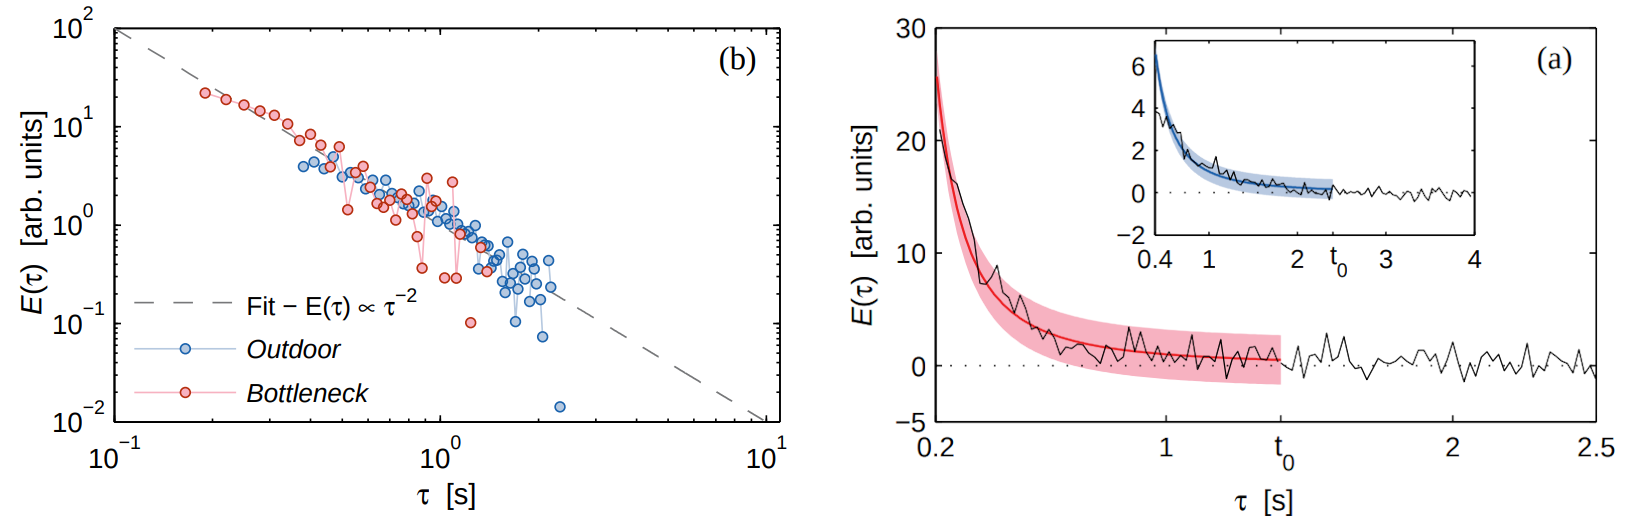
\includegraphics[width=1.0\textwidth]{imgs/pl_graph.png}
  \end{figure}
\end{frame}

\begin{frame}{Powerlaw}
  \begin{itemize}
    \item From that we can generate a model for approximating the energy of a state based on the ttc:
  \end{itemize}
  \begin{gather*}
    E(\tau) = \dfrac{k}{\tau^{2}} e^{-\tau / \tau_{0}}\\\\
    \text{where $\tau$ is the ttc,}\\
    \text{$k$ is a constant that sets the units,}\\
    \text{and $\tau_{0}$ is the time horizon}
  \end{gather*}
\end{frame}

\begin{frame}{Powerlaw}
  \begin{itemize}
    \item This directly implies that the gradient of the energy is the repulsive force experienced by pedestrians
  \end{itemize}
  \begin{gather*}
    \mathbf{F}(\tau) = - \nabla_{\mathbf{r}}\left( \dfrac{k}{\tau^{2}} e^{-\tau / \tau_{0}} \right)\\
    \text{where $\nabla_{\mathbf{r}}$ is the spacial gradient}
  \end{gather*}
  \begin{itemize}
    \item This force is calculated for each agent and combined with a goal driving force
    \item Integrating this force results in a collision free and goal directed velocity
  \end{itemize}
\end{frame}

%------------------------------------------------
\section{Great, now what does that actually mean?}
%------------------------------------------------

\begin{frame}{High Level}
  \begin{itemize}
    \item There is a force driving each agent to the goal
    \item Each agent enacts some sort of force on every other agent
    \item This inter-agent force is sufficient to avoid all collisions between agents
    \item This combination results in a SOTA decentralized motion planning algorithm
  \end{itemize}
\end{frame}

\begin{frame}{Goal Driving Force}
  \begin{itemize}
    \item Defined as the vector pointing directly at the goal
    \item Can be scaled to promote collision-free decisions over goal-directed ones
  \end{itemize}
  \[
    \mathbf{F}_{goal} = \mathbf{g} - \mathbf{p}
  \]
\end{frame}

\begin{frame}{Goal Driving Force}
  \begin{figure}
    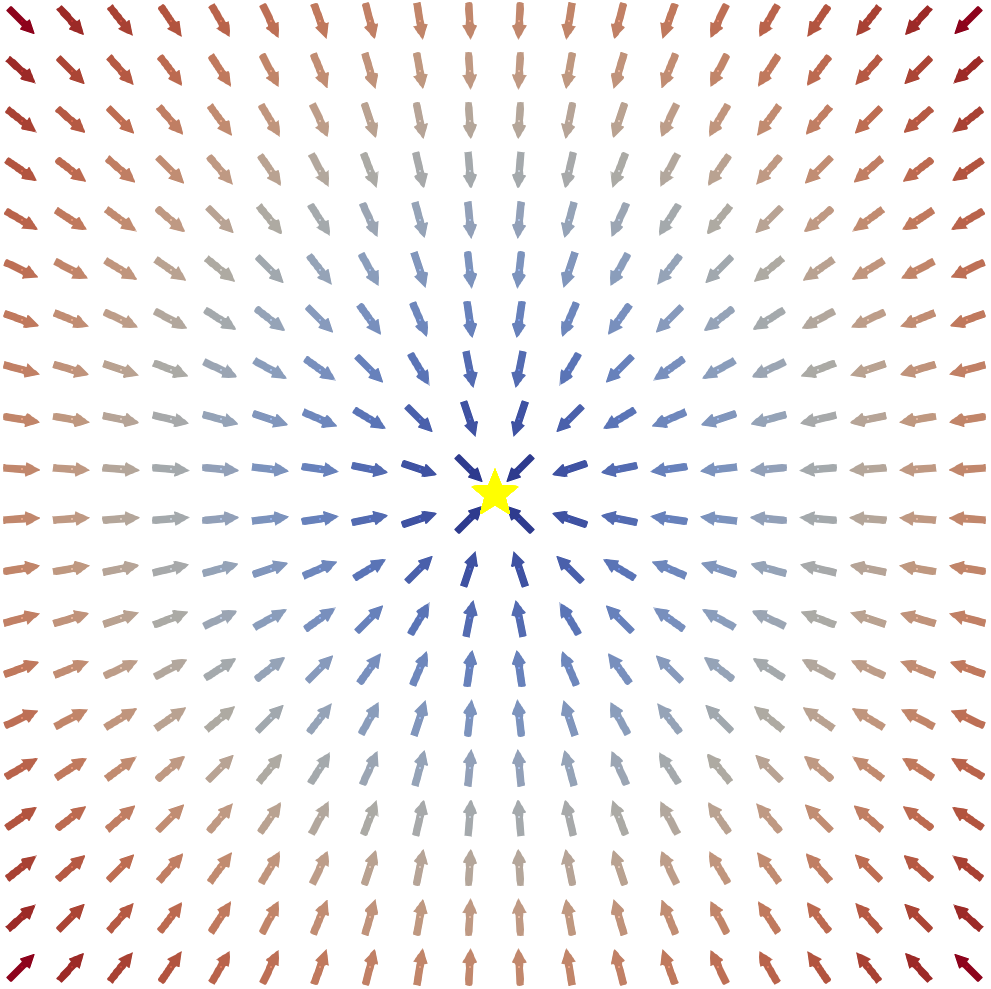
\includegraphics[width=0.5\textwidth]{imgs/goal_directed_force.png}
  \end{figure}
\end{frame}

%------------------------------------------------
\section{Conclusions, Contributions, and Future Work}
%------------------------------------------------

\end{document}
